Il termine \textbf{``sicurezza"} si riferisce alle tecniche, ai processi e ai provvedimenti adottati per proteggere dati, reti di comunicazione, tecnologie informatiche e sistemi di calcolo da attacchi o da accessi non autorizzati. \newline
L'approccio tradizionale prevede che la maggior parte delle risorse a disposizione per mettere in sicurezza il sistema si focalizzi sulle componenti più cruciali e che le protegga dalle minacce più grandi e più note; questo meccanismo fa si che le componenti secondarie siano indifese e, inoltre, non protette da attacchi meno pericolosi. Tale approccio, però, risulta inefficiente nell'ambito della Smart Grid. \newline Per adattarsi al nuovo sistema, le organizzazioni promuovono un metodo più proattivo ed adattivo: il NIST, per esempio, ha recentemente pubblicato delle linee guida che consigliano uno spostamento verso il continuo monitoraggio e verso valutazioni real-time \cite{smartgrids}.\newline \newline
La sicurezza della Smart Grid, in relazione al suo sviluppo, è un tema fortemente discusso: tutti concordano nel sostenere che la Smart Grid dovrebbe avere un modello di sicurezza robusto; il problema è che ci si trova dinanzi a due sfide: come poter rispondere ai requisiti richiesti e come poter applicare le numerose alternative esistenti quando si cerca di rendere sicuro un ambiente complesso come la Smart Grid.
\newline \newline
Quando si sente parlare di ``nuova tecnologia", di ``interconnessione" e di ``condivisione dei dati", subito ci si focalizza sui benefici e sulle nuove funzionalità che tali concetti portano con loro. C'è da considerare, però, anche i nuovi rischi che queste nuove funzionalità introducono all'interno del sistema.\newline Per questo motivo, lo scopo della sicurezza è quello di garantire che le funzionalità del sistema operino correttamente e siano protette da abusi. È importante sottolineare, però, che non esistono applicazioni, reti o sistemi completamente sicuri e le Smart Grid non sono un'eccezione. Sebbene ogni componente della nuova rete elettrica porti con se numerosi miglioramenti operazionali  o funzionali, introduce anche nuove vulnerabilità e rischi addizionali che, se non propriamente gestiti, possono portare il sistema ad essere esposto ad attacchi di varia natura.
\section{Un caso esemplare di attacco: Stuxnet}
Stuxnet è un noto worm di 500 Kbyte scoperto nel 2010 da VirusBlokAda, una società di sicurezza bielorussa. Un \emph{worm} è una particolare categoria di malware in grado di autoreplicarsi. È simile ad un virus ma, a differenza di questo, si diffonde spedendosi direttamente agli altri computer, ad esempio tramite e-mail o in una rete.  Stuxnet ha infettato il software di almeno 14 siti industriali in Iran, tra cui un impianto di arricchimento dell'uranio. Questo pezzo di codice maligno ha attaccato in tre fasi. In primo luogo attaccava macchine Windows e reti, replicandosi ripetutamente. Poi passava alla ricerca del software Siemens Step7 che è Windows-based e utilizzato per programmare sistemi di controllo industriale e infine comprometteva i programmable logic controller. La Figura \ref{fig:stxhsw} mostra il modo in cui opera Stuxnet.
\begin{figure}[h]
	\centering
	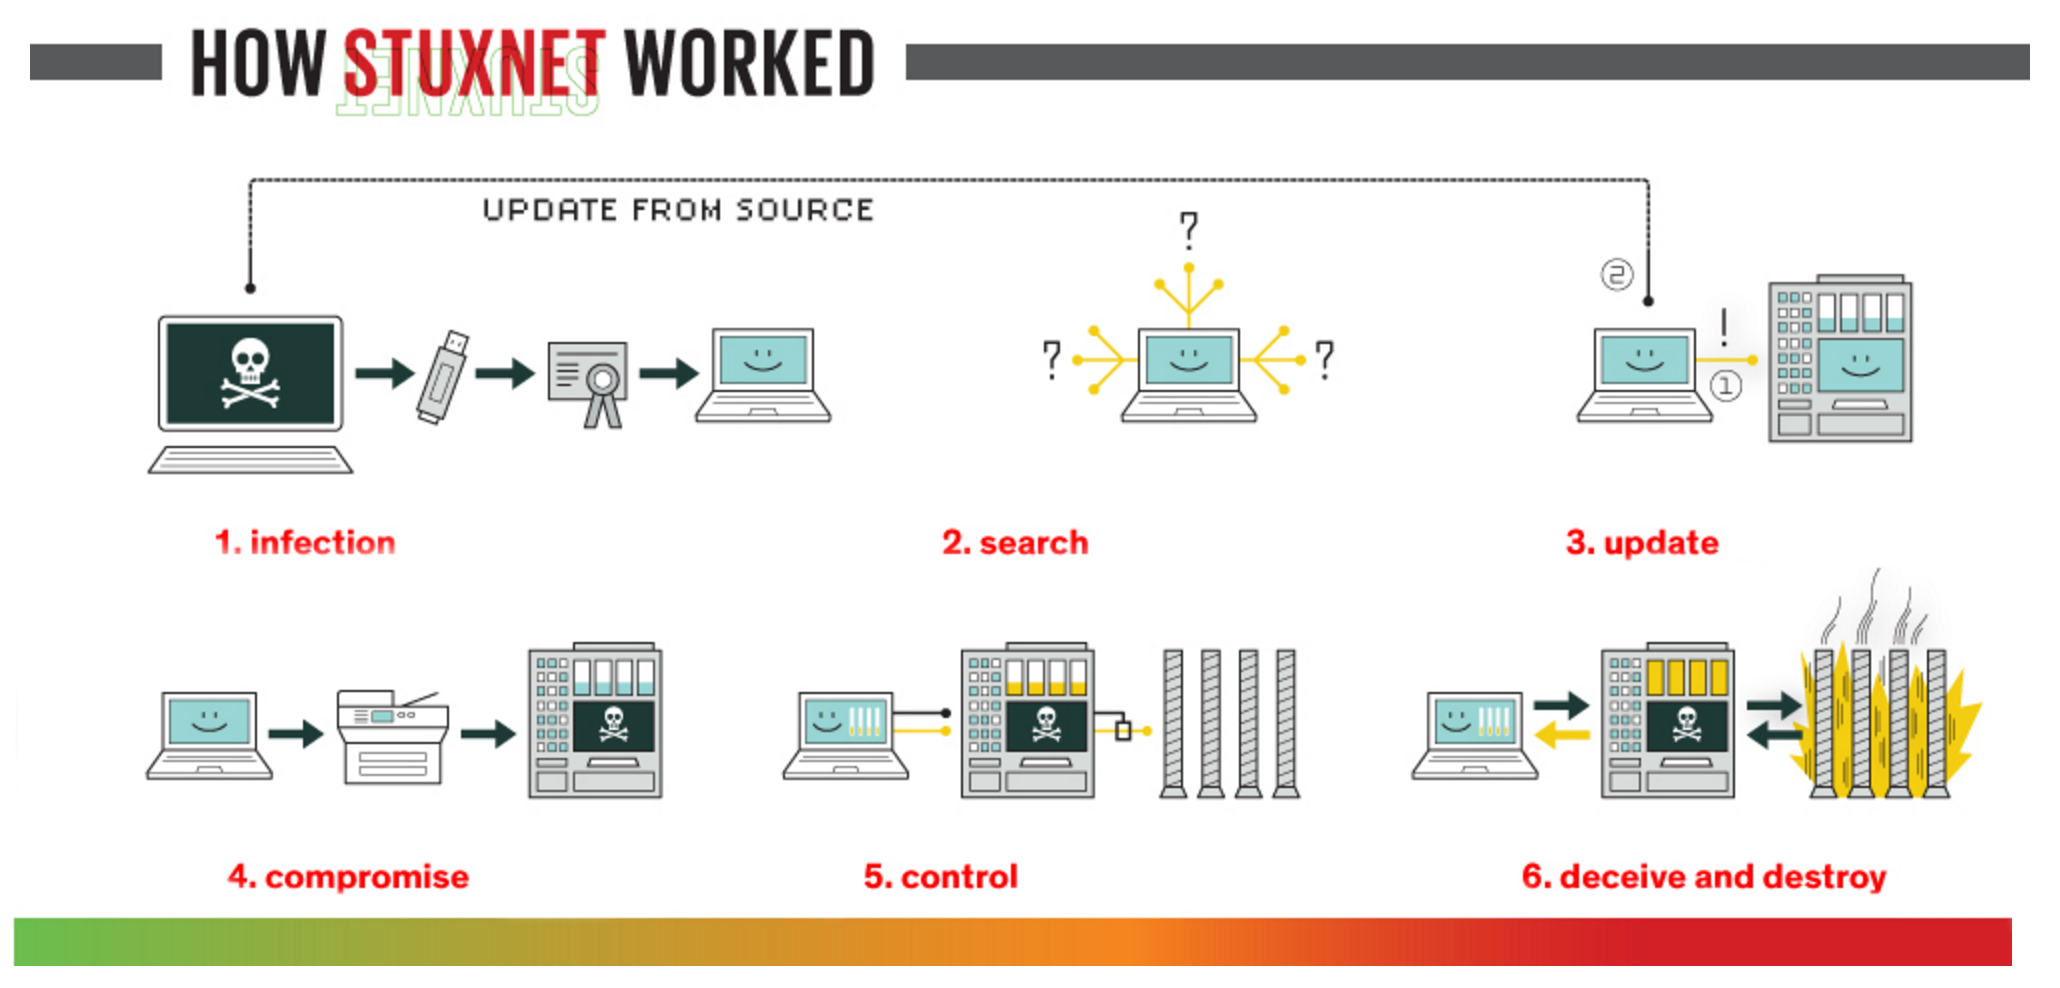
\includegraphics[scale=0.350]{imgs/stuxnet_hsw.png}
	\caption{}\label{fig:stxhsw}
\end{figure}
\begin{enumerate}
	\item\emph{Infection}: stuxnet entra nel sistema attraverso il collegamento di una penna USB e procede con l'infettare tutte le macchine su cui gira Microsoft Windows. Grazie all'utilizzo di un certificato digitale che lo fa sembrare affidabile, il worm è in grado di eludere sistemi di automated-detection;
	\item\emph{Search}: stuxnet verifica se una macchina è parte del sistema di controllo industriale creato da Siemens;
	\item\emph{Update}: se il sistema non è target, Stuxnet non fa niente; in caso contrario, il worm prova ad accedere ad Internet e scaricare una versione più recente di se stesso.
	\item\emph{Compromise}: il worm quindi compromette i controllori logici del sistema target, sfruttando la vulnerabilità ``zero day'';
	\item\emph{Control}: in principio, si spiano le operazioni del sistema target. Successivamente, si usano le informazioni raccolte per prendere il controllo delle centrifughe, portandole al deterioramento;
	\item\emph{Deceive and Destroy}: fornisce false informazioni ai controllori, assicurando che questi ultimi non si accorgeranno del problema fin quando non sarà troppo tardi per fare qualsiasi cosa.
\end{enumerate}
Stuxnet è stato creato e diffuso dal governo USA in collaborazione col governo Israeliano nella centrale iraniana di Natanz, allo scopo di sabotare la centrifuga della centrale tramite l'esecuzione di specifici comandi da inviarsi all'hardware di controllo industriale responsabile della velocità di rotazione delle turbine allo scopo di danneggiarle. Stuxnet si diffondeva velocemente sulle macchine che utilizzavano Windows, pur non essendo collegati ad Internet. Un operaio che inseriva una penna USB in una macchina infetta poteva propagare inconsapevolmente il worm sulla macchina che leggeva successivamente dalla stessa penna. Data la facile diffusione, gli esperti temevano che il malware poteva propagarsi anche su scala mondiale.\newline\newline
Gli autori di Stuxnet non sono stati identificati ma dalla sua scoperta gli ingegneri di sicurezza informatica stanno combattendo contro altre cyber-armi che sono state considerate varianti rispetto all'originale Stuxnet, fra queste Duqu e Flame. Mentre Stuxnet aveva lo scopo di ``distruggere'', lo scopo di Flame era solo quello di ``spiare''. Una volta che Flame aveva compromesso una macchina, era in grado di cercare delle keyword su file PDF top-secret e/o trasmettere parti del documento, il tutto senza essere scoperti.\newpage
Inoltre, Flame non trasmetteva le informazioni raccolte tutte in una volta al suo server, in quanto il network manager poteva notare questo grande flusso improvviso di dati. L'idea, era quindi, quella di spedire i dati in blocchi di piccola dimensione per evitare di monopolizzare la larghezza di banda disponibile per troppo tempo. Siemens, dopo qualche tempo ha messo a disposizione uno strumento per il rilevamento e la rimozione di Stuxnet. Ha richiesto inoltre agli utenti di evitare l'utilizzo di penne USB non sicure all'interno della rete anche nel periodo successivo alla rimozione del virus. Uno strumento gratuito per la rimozione di Stuxnet è messo a disposizione da BitDefender sul suo sito dedicato \url{MalwareCity.com}.
\section{Definire la sicurezza}
La sicurezza tradizionale fa affidamento sulla cosiddetta \textbf{CIA triad}, che ne costituisce il cuore. La CIA triad comprende tre concetti: \emph{confidentiality}, \emph{integrity} ed \emph{availability}. \newline Una concezione più moderna, e più adatta all'ambiente della Smart Grid, prevede l'utilizzo del \textbf{Parkerian hexad}, figura \ref{fig:31}, proposto da Parker nel 2002. Tale modello propone, in aggiunta ai tre classici concetti precedenti, altri tre principi: \emph{control} (o \emph{possession}), \emph{authenticity} ed \emph{usability} (o \emph{utility}). \newline All'interno di questi sei pilastri, è possibile trovare tutti i problemi relativi alla Smart Grid \cite{smartgrids}.
\begin{figure}[h]\centering{
  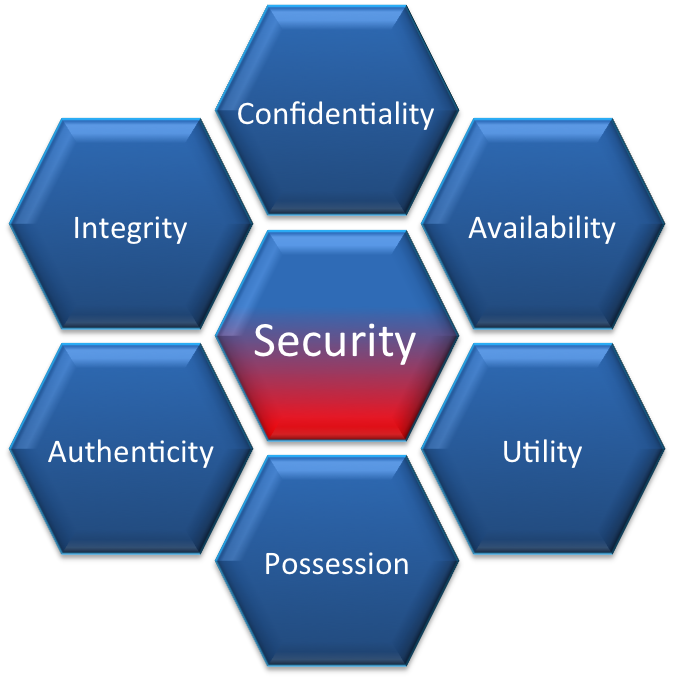
\includegraphics[scale=0.5, natwidth=674,natheight=679]{imgs/hexad.png}
  \caption{Parkerian hexad}\label{fig:31}
}
\end{figure}
\subsection{Confidentiality}
Tale concetto porta con sé una serie di problemi e di preoccupazioni relative alla trasmissione e alla memorizzazione di dati ricavati dalle operazioni della Smart Grid. Questo tipo di dati, infatti, è spesso ritenuto \textit{confidenziale}, nel senso che se fosse noto, avrebbe tutto il potenziale per causare danni alla sicurezza delle operazioni di tutto il sistema. \newline La confidenzialità, inoltre, può essere intesa anche in un'altra accezione: se i dati fossero noti alla concorrenza, per esempio,  quest'ultima potrebbe trarre un notevole vantaggio in uno specifico settore o in tutto il mercato. \newline A tali fattori si aggiungono altre nuove problematiche legate alla \textit{privacy del consumatore} e, quindi, dei suoi dati, che vengono fuori da meccanismi di metering quali l'AMI. Gli utenti, infatti, si aspettano che i consumi relativi alle loro abitazioni private rimangano confidenziali; se così non fosse, la disponibilità di tali informazioni insieme alla capacità di fare data mining, avrebbe il potenziale per creare significative preoccupazioni sulla privacy. \newline I punti della Smart Grid che introducono rischi per la confidenzialità, sono costituiti da tutte le locazioni in cui sono memorizzati i dati e da tutti i meccanismi di trasmissione delle informazioni. Per quanto riguarda i dati memorizzati, questi potrebbero essere letti, copiati e distribuiti a soggetti diversi dai destinatari. Per quanto riguarda la trasmissione, invece, sia su reti private che su reti pubbliche come Internet, i dati potrebbero essere intercettati, copiati e distribuiti. \newline La soluzione a tali problemi risiede nelle funzioni di \textit{cifratura dei dati} e di \textit{controllo degli accessi}. Fornendo l'appropriato livello di cifratura delle informazioni, quest'ultime possono essere protette da chiunque non sia il diretto destinatario. \newline Il controllo degli accessi, prevede che i dati siano protetti da coloro che hanno l'autorizzazione per accedere al sistema ma che, allo stesso tempo, non hanno bisogno di tali dati per svolgere il loro lavoro.

\subsection{Integrity}
L'integrity si riferisce all'abilità del sistema di evitare che le informazioni possano essere modificate da persone o da sistemi non autorizzati. \newline Se si rendono possibili meccanismi di modifica volontari quali la manipolazione dei dati, o anche involontari quali la loro corruzione, i sistemi riceveranno informazioni non accurate; a lungo andare ciò potrebbe avere un impatto negativo su tutte le operazioni e, in casi estremi, portare ad instabilità o compromettere del tutto la Smart Grid. \newline
I punti della nuova rete elettrica che introducono rischi per l'integrità, sono tutti quei punti che consentono il passaggio dei dati da un sistema ad un altro. Pertanto, la sicurezza di tali meccanismi di transizione è importante, ma ancora più importante è come il sistema che riceve i dati possa assicurarsi della validità di quest'ultimi: se i dati subiscono manipolazioni mentre sono in viaggio tra i due sistemi, il ricevente potrebbe prendere decisioni basate su tali informazioni (che risultano essere errate); se, invece, i dati sono soggetti a corruzione durante la loro transizione, ci si potrebbe trovare di fronte ad un comportamento inaspettato del ricevente. In entrambi i casi, è evidente che l'integrità dei dati sia cruciale per assicurare la stabilità delle operazioni.   \newline
Le risposte ai problemi di integrità, possono essere trovate nei meccanismi di \textit{auditing}, di \textit{authorization}, di \textit{nonrepudiation}, e di \textit{message-signing}, che saranno trattati in seguito (vedi Paragrafo 4.3).


\subsection{Availability}
Molto spesso si tende ad utilizzare i concetti di reliability ed availability in maniera intercambiabile; in realtà, tali concetti hanno due significati diversi. La reliability, infatti, risponde alle seguenti domande: ``quanto spesso fallisce il sistema?", ``quanto è elastico?"; l'availability, invece, indica la disponibilità del sistema e, quindi, la capacità di compiere il lavoro che gli è stato assegnato, \textit{nel momento in cui se ne ha bisogno}. \newline Una porzione del sistema potrebbe essere attiva, eseguendo e processando i comandi, il 100\% del tempo, e pertanto molto affidabile ma, se le performance non sono adeguate ai bisogni della rete e operazioni critiche vengono ritardate o mancano, non si può dire che il sistema sia disponibile. \newline
I punti della Smart Grid che introducono rischi per la disponibilità sono troppi per poterli elencare: qualsiasi sistema, rete, dispositivo che gestisce le comunicazioni, processo per la gestione dei messaggi, e qualsiasi servizio invocato a qualsiasi livello applicativo e il suo sistema operativo sottostante sono un rischio per la disponibilità quando si trovano a dover gestire l'inoltro di un comando da un'estremità del sistema ad un'altra. Risolvere tale rischio è quasi tanto complicato quanto identificare le componenti del sistema che hanno il potenziale per impattare sulla disponibilità. La maggior parte delle soluzioni si affida a tecniche di ridondanza (clustering, bilanciamento del carico); il costo di tali metodologie, però, cresce in maniera proporzionale ai punti di fallimento che si identificano nel sistema. 

\subsection{Control}
La capacità di controllare le informazioni che necessitano protezione è essenziale per assicurare la loro integrità e la loro usabilità a lungo termine. Ciò ha diverse implicazioni per tutti quei sistemi che si affidano al meccanismo di controllo per scopi di vario genere (legali, normativi o commerciali): se le informazioni utilizzate per calcoli finanziari, come ad esempio i dati ricavati da meccanismi di metering, non fossero controllate, potrebbero compromettere tutti i sistemi che le forniscono e le trasmettono; di conseguenza, la provenienza di tali informazioni non potrebbe essere più garantita, portando una diminuzione dell'affidabilità di quest'ultime. 

\subsection{Authenticity}
Tale termine è spesso utilizzato per descrivere la certezza della provenienza. Il processo di verifica dell'autenticità è simile al processo utilizzato per verificare l'integrità: assicurarsi che la fonte dei dati e i dati stessi, siano autentici.

\subsection{Usability}
Questo aspetto del Parkerian hexad si preoccupa di assicurare che i dati siano utilizzabili. \newline Consideriamo un flusso di dati opportunamente cifrato: quest'ultimo garantisce la sicurezza delle informazioni, ma rende molto difficile far si che queste ultime siano utili. L'usabilità è il fattore che, in definitiva, fornisce valore a livello aziendale e pertanto deve essere preservato e trattato come il requisito con più alta priorità. 

\subsection{Analisi dei rischi}
Quale sarebbe il rischio per l'intero sistema Smart Grid se il sistema stesso, o qualsiasi sua componente, fosse compromessa? Tale rischio e il suo potenziale costo, guidano il lato economico delle decisioni per la progettazione dei meccanismi di sicurezza. \newline Come determinare l'accettazione dei rischi è, pertanto, una decisione legata al business e non una decisione tecnica. Un'azienda che sceglie di adottare una particolare metodologia per l'analisi dei rischi, avrà come input le proprie variabili che guidano le decisioni; tali variabili sono solitamente legate ad un rischio finanziario che l'azienda assume basandosi su una propria analisi competitiva del mercato o su condizioni regolamentari sotto le quali opera. \newline Ci sono altre motivazioni, oltre a quelle finanziarie, che possono guidare l'accettazione dei rischi, come ad esempio fattori legislativi o legati a normative industriali: tali fattori possono portare ad adottare comportamenti che garantiscono la sicurezza anche in assenza di forti incentivi economici, per aggiungere ulteriori capacità di protezione del sistema. \newline È importante riconoscere che nessuna decisione riguardante la sicurezza dovrebbe essere presa senza prima aver considerato i rischi: ``dove sono i rischi nel sistema?", ``Quanto costerà un fallimento del sistema?", ``Quanto costerà un fallimento della sicurezza del sistema?". Un'azienda dovrebbe essere in grado di capire i rischi e dovrebbe essere capace di fare scelte informate ed intelligenti su come risolvere tali problemi. 


\section{Building blocks}
Nel paragrafo precedente, sono state descritte una serie di potenziali minacce e funzioni di sicurezza che sono importanti per sistemi complessi ed interdipendenti come le Smart Grid. \newline In questo paragrafo, si esaminerà una possibile architettura di sicurezza che comprende tutte le funzioni precedentemente analizzate e che cerca di creare una struttura adatta a risolvere tutte le vulnerabilità descritte nel Paragrafo 4.2.

\subsection{Layered Security Model}
Il concetto di modello di sicurezza \textit{stratificato} non è un concetto nuovo: i sistemi operativi ed i microprocessori, infatti, lo utilizzano da tempo per controllare gli accessi a  risorse privilegiate. \newline Immaginare tale concetto applicato ad una Smart Grid non è difficile. \newline Dalla figura \ref{fig:32} è possibile vedere che la struttura di tale modello è una struttura ad anello in cui la comunicazione tra gli strati del sistema è sicura. In generale, uno strato esterno non può avere libero accesso alle risorse presenti su uno strato più interno; inoltre, le richieste per le risorse non dovrebbero essere in grado di ``saltare" i vari anelli: una richiesta che parte dal terzo anello, non dovrebbe poter accedere direttamente alla risorsa del primo, ma gli accessi sono regolati da opportune interfacce progettate in modo tale da assicurare la sicurezza di tutto il sistema.

\begin{figure}[h]\centering{
  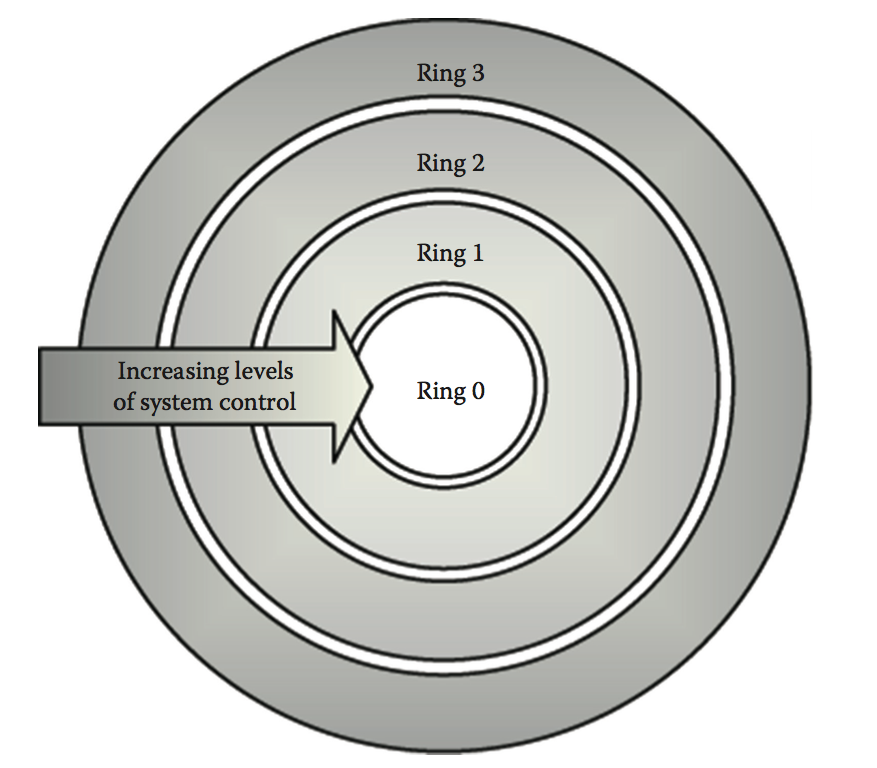
\includegraphics[scale=0.25, natwidth=877,natheight=768]{imgs/ring.png}
  \caption{Layered security model}\label{fig:32}
}
\end{figure}

Una Smart Grid ben progettata, dovrebbe essere in grado di offrire una simile protezione: i sistemi e le risorse poste agli estremi, come ad esempio dispositivi HAN (home area network) o smart meter, non dovrebbero avere la possibilità di accedere direttamente agli strati operativi (ring 0) della Smart Grid e, in più, i dati che passano per il sistema dovrebbero attraversare opportune interfacce che ne assicurino l'integrità prima di procedere verso strati più interni. \newline
Indipendentemente dal meccanismo specifico utilizzato per separare gli strati, ci sono diversi principi architetturali chiave che dovrebbero essere considerati nel percorso dei dati tra gli anelli: il primo e il più importante è assicurarsi che un fallimento in uno strato non abbia impatto né in uno strato più basso né in qualsiasi sistema dello stesso strato. Con il termine ``impatto" ci si riferisce al fatto che nessuna tra confidentiality, integrity, o availability degli strati sottostanti debba essere colpita. È importante notare, però, che il viceversa non è vero: molto spesso danni ai livelli più bassi si propagano verso gli strati superiori e ciò è dovuto alla natura gerarchica del sistema.
\newline \newline 
Nelle prossime sezioni si analizzano le principali funzioni che costituiscono le componenti di sicurezza di alto livello che la Smart Grid dovrebbe avere per assicurare la protezione del sistema.

\subsection{Authentication}
L'autenticazione è il processo di verifica dell'identità di una persona o di un servizio che richiede l'accesso ad una risorsa. \newline Un meccanismo di autenticazione robusto potrebbe richiedere un certo numero di componenti, ognuna delle quali offre una particolare funzione di tutto il processo. \newline Spesso si tende a pensare all'autenticazione in termini di username e password, il che è corretto, ma non è solo questo: vi può essere autenticazione anche tra sistemi, processi o componenti hardware. Ci sono due componenti base per un meccanismo di autenticazione:
\begin{itemize}
\item \textit{Identity Database}, contiene le informazioni necessarie per determinare chi e cosa sta tentando di accedere al sistema;
\item \textit{Identity Management System}, repository centrale di tutte le risorse che richiedono servizi di autenticazione.
\end{itemize}

\subsection{Authorization}
L'autorizzazione è il processo che verifica ciò che la persona o il servizio autenticato può fare all'interno del contesto del sistema. \newline 
Spesso i sistemi più semplici prevedono solo due modalità: ``read-write" e ``write-only"; i sistemi più complessi, invece, dovrebbero fornire regole di autorizzazione più specifiche, includendo la possibilità di indicare quali campi si possono modificare e quali no, solo ad un certo orario del giorno e solamente se autenticati su specifiche macchine.

\subsection{Auditing}
Il cuore di una qualsiasi analisi dei rischi è costituito dal programma di controllo. Senza revisioni periodiche dell'efficacia dei meccanismi di sicurezza che sono in atto nella Smart Grid, non ci sarebbe nessuna garanzia che il sistema sia sicuro. \newline
Un buon programma di controllo dovrebbe essere eseguito periodicamente e dovrebbe testare quelle componenti che sono ritenute essenziali dall'azienda per mettere in sicurezza le operazioni del sistema. Tra i meccanismi più utili per eseguire tali revisioni, vi sono i seguenti:
\begin{itemize}
\item \textit{Logging}: utilizzare file di log e memorizzare al loro interno tutti gli accessi critici al sistema e tutti i cambiamenti avvenuti;
\item \textit{Time Synchronization}: in un sistema unificato come una Smart Grid, è essenziale che tutti i dispositivi condividano lo stesso tempo.
\end{itemize}

\subsection{Key Management}
È il processo che gestisce le emissioni delle chiavi per utenti, applicazioni e dispositivi. Tali chiavi sono utilizzate per stabilire l'identità e per assicurare l'integrità dei messaggi quando si inviano comandi tra sistemi. \newline 
Se consideriamo centinaia di chiavi, la loro gestione è relativamente semplice; ma quando ci si trova di fronte a centinaia di migliaia, o addirittura milioni, di dispositivi, la gestione diventa più complessa. Ogni chiave nel sistema sia relativa ad applicazioni, al sistema, ad un dispositivo o ad una persona, dovrebbe poter essere modificata o revocata su richiesta. 
\newline Per fare ciò, si utilizza la ben nota \textit{Public Key Infrastructure} (PKI) \cite{smartgrid}.

\subsection{Message Integrity}
Per trattare l'integrità dei messaggi, consideriamo tre meccanismi: signing, nonrepudiation ed encryption. \newline
Per quanto riguarda il meccanismo di \textit{signing}, quando un messaggio viene inviato da un sistema ad un altro, vi è prima un processo di autenticazione per dimostrare un'identità, seguito da un processo di autorizzazione, per verificare ciò che l'identità può fare. Una volta effettuati questi due controlli, può iniziare lo scambio di messaggi tra i due sistemi. Ci sono due motivazioni principali per cui conviene firmare un messaggio: la prima è assicurare che il contenuto del messaggio non sia stato modificato durante la trasmissione tra i sistemi; la seconda è permettere di verificare l'identità del mittente indipendentemente dal processo di autenticazione. \newline
La \textit{nonrepudiation} entra in gioco quando il mittente di un messaggio necessita di essere riconosciuto (o confermato). Tale termine, infatti, si riferisce alla capacità di fornire una prova inconfutabile, ad una terza parte, di chi ha iniziato una certa azione nel sistema, anche se la persona in questione non sta partecipando al momento. \newline
Il termine \textit{encryption} porta con sé una serie di problematiche e di discussioni ampiamente trattate in letteratura, pertanto è impossibile riassumerlo in poche righe. Si può, però, riassumere il suo scopo: assicurarsi che un messaggio non possa essere letto da una persona o da un sistema che non sono i diretti destinatari dell'informazione. Ciò può essere messo in pratica attraverso innumerevoli algoritmi di cifratura, i quali fanno affidamento sul preservare l'integrità della chiave utilizzata per cifrare i dati; pertanto se tale chiave viene compromessa, lo sarà anche il messaggio. 

\subsection{Network Integrity}
Vi è un'infinità di modi per garantire l'integrità di rete, ognuno dei quali dipende dai dispositivi che la compongono e dalle loro necessità. Infatti, poiché ogni rete ha bisogni diversi, non vi è una configurazione che sia adatta a tutte quante.
\newline Due dei meccanismi principali sono i seguenti:
\begin{itemize}
\item \textit{Firewall}, utilizzato per restringere il traffico sulla rete ad uno specifico insieme di regole. Per esempio, potrebbe limitare il traffico a specifici canali di comunicazione tra un dispositivo e un insieme noto di altri dispositivi;
\item \textit{Rilevamento e prevenzione delle intrusioni}, messo in atto analizzando il traffico della rete per identificare specifici pattern di dati che corrispondono ad attacchi noti.
\end{itemize}

\subsection{System Integrity}
\begin{itemize}
\item \textit{Protezione da malware}, o più comunemente nota come protezione antivirus: ogni sistema dovrebbe avere una strategia che lo protegga da questo tipo di minacce; una protezione robusta, infatti, non solo può evitare che file maliziosi vengano memorizzati, ma può anche far si che si possa avvisare un operatore del ritrovamento del malware;
\item \textit{Gestione della configurazione del sistema}: le specifiche su come un sistema è configurato possono impattare enormemente sulla sua sicurezza. La gestione è necessaria per assicurarsi che il sistema non cambi rispetto alle basi di funzionamento stabilite;
\item \textit{Validazione e testing}: essenziali per garantire l'integrità del sistema. Prima di effettuare qualsiasi cambiamento e di distribuire nuovi sistemi, bisogna valutare le nuove modifiche e capire che impatto hanno sull'intero sistema. I cambiamenti devono essere testati per sicurezza e per garantire che non abbiano conseguenze negative sull'affidabilità di tutto il sistema.
\end{itemize}

\section{Threats and Impacts}
Analizziamo ora le minacce a cui una Smart Grid può essere sottoposta e l'impatto che esse hanno sull'infrastruttura, focalizzandoci principalmente su due attori del sistema: gli utenti e le società di servizi. Maggiori dettagli possono essere trovati in \cite{securingSG}.
 
\subsection{Consumers threats}
Il fatto che gli utenti si trovino ad affrontare le minacce poste dalle nuove tecnologie non è un qualcosa di nuovo. Essi, infatti, sebbene non sia esattamente la stessa situazione, si sono già trovati di fronte a problemi simili introdotti dai personal computer, dai  cellulari e dall'attuale rete elettrica: man mano che aumenta la dipendenza dalla tecnologia, così aumenta anche la dipendenza dalla corrente elettrica per alimentare la tecnologia. Nel momento in cui ad una persona, però, viene sottratto un apparecchio tecnologico, riuscirà a sopravvivere anche senza; ma, se alla stessa persona viene negato l'accesso alla corrente elettrica, il danno che essa ne subirà sarà sicuramente maggiore.\newline
Gli utenti di una Smart Grid possono essere sottoposti ad una serie di pericoli di varia natura, partendo dalla privacy fino ad arrivare a situazioni che rischiano di mettere in pericolo la loro stessa vita:
\begin{itemize}
\item \textit{Minacce naturali}. In accordo al \textit{NERC Disturbance Analysis Working Group} (DAWG) \cite{securingSG}, i disastri metereologici e naturali (quali venti, tempeste, tornadi, terremoti, ecc.) sono la causa di più del 50\% dei disturbi del sistema elettrico e, in particolare, degli utenti. La Smart Grid si propone di affrontare tali minacce ma è importante notare che eliminare totalmente i danni causati dai frequenti disastri atmosferici e naturali non è fattibile in maniera semplice nel prossimo futuro. Poichè non si può fermare il verificarsi di tali calamità, i programmi di aiuto in caso di incidenti continueranno ad essere di critica importanza, in risposta ai fenomeni naturali distruttivi;
\item \textit{Minacce provenienti da singoli o da organizzazioni}. L'AMI e gli altri componenti della Smart Grid, permettono agli operatori di amministrare da remoto i dispositivi situati nelle case degli utenti; in più gli \textit{smart device}, permettono ai consumatori e alle società di servizi di controllare in maniera remota anche i consumi energetici. Numerose sono le motivazioni che possono spingere persone e organizzazioni ad abusare delle funzionalità di questi dispositivi; la possibilità di ottenere il controllo di tali componenti, può portare ad attaccare la Smart Grid e, quindi, i suoi utenti. Varie possono essere le figure coinvolte in tali situazioni:
	\begin{itemize}
	\item \textit{Ladri e stalker}. Uno degli obiettivi della Smart Grid, come detto nei capitoli precedenti, è quello di rendere gli utenti più consapevoli dei propri consumi e, in questo modo, aiutarli a cambiare i propri comportamenti energetici allo scopo di ridurre i costi delle bollette. Ma, l'accesso a tali informazioni, può far sì che altre persone possano compiere azioni maliziose: supponiamo che un ladro riesca a monitorare il consumo elettrico di una certa abitazione; tale persona può rendersi conto, in base agli orari di attività e inattività della corrente e ai consumi in ciascun orario, delle abitudini quotidiane degli inquilini di tale abitazione. Se riesce a monitorare questi comportamenti per un periodo di tempo ampio, riuscirà ad individuare quando le persone non sono in casa e potrà, quindi, compiere un furto all'interno dell'abitazione, oppure, riuscendo ad individuare i momenti di utilizzo di energia settimanali e giornalieri, potrà utilizzare la loro corrente per i suoi scopi. Uno stalker, analogamente, analizzando i consumi di un veicolo elettrico di una determinata donna, può essere in grado di individuare i suoi spostamenti e le sue abitudini;
	\item \textit{Hacker}. I motivi per ``hackerare" una Smart Grid possono essere vari. Tra i principali ci sono sicuramente motivi non maliziosi: una persona potrebbe essere semplicemente curiosa di capire come funziona un determinato dispositivo, oppure potrebbe utilizzare la Smart Grid come un mezzo per ottenere gratificazione personale o per egoismo; sebbene tali motivazioni non siano maliziose, possono comunque arrecare danno all'infrastruttura. Un'altra causa che spinge ad hackerare la rete potrebbe essere un semplice test per verificare la robustezza del programma di sicurezza e per indentificare, quindi, le potenziali vulnerabilità. Le persone che effettuano tali test, ovviamente fanno il possibile per evitare che il loro lavoro abbia conseguenze negative sul sistema elettrico. In aggiunta a tali motivazioni, però, esistono giustificazioni per l'attacco della rete tutt'altro che non maliziose: guadagno economico, desiderio di potere, sete di vendetta e volontà di distruggere il sistema;
	\item \textit{Terrorismo}. A prescindere dalle motivazioni e dalla categoria di attacco, le Smart Grid sono considerate potenziali target per i terroristi. Attaccando la  rete elettrica, i terroristi potrebbero colpire enormi quantità di persone e, come risultato, spostare verso di loro un'attenzione massiva;
	\item \textit{Gorverno}. Il governo è sia un consumatore, che una minaccia per i consumatori: dai semafori stradali ai laboratori di ricerca, le agenzie governative consumano una grande quantità di energia e, pertanto, sono anche loro suscettibili ai pericoli visti in questo paragrafo. Nonostante ciò, il governo può anche rappresentare una minaccia per gli utenti, in particolare su due aspetti: la guerra e le attività illegali. Per quanto riguarda la guerra, è normale pensare che paralizzare un'infrastruttura critica nazionale come la rete elettrica possa ostacolare le capacità della nazione stessa di operare; per questo motivo la Smart Grid è uno dei target durante la guerra. Per quanto riguarda le attività illegali, come ad esempio la produzione di droga, spesso queste fanno uso di energia elettrica per poter andare avanti. Utilizzando una rete intelligente, è possibile, monitorando i consumi di tali attività, riuscire ad individuare le operazioni illegali che effettuano, localizzare dove esse avvengono e arrestare i colpevoli;
	\item \textit{Società di servizi}. Tali società, o più precisamente i suoi agenti, possono essere una minaccia per i consumatori attraverso azioni intenzionali e non intenzionali. A partire dagli incidenti fino alle minacce interne, tali persone possono continuare ad essere la causa di interruzioni di corrente,  \textit{privacy leak}, fatturazioni improprie e altro.
	\end{itemize}
\end{itemize}

\subsubsection{Impatti}
Le minacce e i problemi visti nel paragrafo precedente, possono comportare una serie di danni e di conseguenze differenti; i principali sono:
\begin{itemize}
\item \textit{Impatto sui consumatori}. In questo caso è la privacy che, in particolare, subisce le maggiori conseguenze: nell'implementazione dell'AMI, gli \textit{smart meter} collezionano in maniera autonoma un grande ammontare di dati e lo trasportano alle società di servizi, al cliente e ai fornitori di servizi di terze parti. Tali dati includono anche informazioni personali identificative che possono, quindi, compromettere la privacy del cliente. Pertanto un tale dettaglio nel resoconto dei consumi di una persona, può far si che altre persone e organizzazioni riescano a tracciare un profilo delle abitudini. Se tali informazioni giungono ad un hacker, come detto in precedenza, lui potrà utilizzarle per scopi maliziosi; se, invece, giungono nelle mani di servizi di terze parti affidabili, quali agenzie pubblicitarie, esse ne potranno fare un uso più leggittimo;
\item \textit{Impatto sull'availability}. Al di là di tutte le nuove funzionalità e le nuove caratteristiche introdotte, l'obiettivo principale di una Smart Grid rimane quello di rendere la corrente sempre disponibile ai clienti. Pertanto, la maggior parte dei pericoli analizzati precedentemente, può incidere sulla disponibilità di energia. Gli impatti che ciò può avere sul sistema variano dall'alterare i termostati che regolano riscaldamento e aria  condizionata, fino a limitare, o addirittura impedire, servizi di emergenza;
\item \textit{Impatto finanziario}. I pericoli sopra descritti possono avere serie conseguenze sulle finanze dei clienti: corrompere i dati che nascono dagli \textit{smart meter}, può portare al calcolo di bollette non accurate che, di conseguenza, comporta un pagamento da parte degli utenti maggiore del loro effettivo consumo.
\end{itemize}

\subsection{Utility companies threats}
Alcuni dei pericoli a cui le società di servizi possono essere esposte sono simili alle minacce riguardanti i consumatori, altri sono unici, ma la cosa certa è che attaccare tali compagnie, le aziende e i governi avrà un impatto più grande degli attacchi contro gli utenti. \newline In questo paragrafo, verranno analizzate le minacce che impattano sulle componenti della \textit{CIA triad} relative alle società, mostrando per ognuna di esse uno scenario ipotetico e le conseguenze.

\subsubsection{Confidentiality}
Come detto nel paragrafo 4.2, si soddisfa il requisito di \textit{confidentiality} nel momento in cui si proteggono i dati da accessi non autorizzati: la perdita tale requisito arreca un grande danno ai consumatori, ma rende anche le società di servizi un \textit{target} molto appetibile per gli hacker, in quanto tali società effettuano aggregazione di informazioni personali. Gli attacchi possibili riguardano i seguenti ambiti:
\begin{itemize}
\item \textit{Privacy del consumatore}. Le società di servizi raccolgono e memorizzano varie informazioni personali dei clienti (e.g. nome, indirizzo, dati relativi ai consumi), informazioni che ci si aspetta restino confidenziali. Fare breccia nella confidenzialità per accedere a tali dati è l'obiettivo di molti hacker; tuttavia, non sono solo loro a poter volere tali informazioni. Le nuove tecnologie introdotte dalla Smart Grid permettono agli utenti di interagire più frequentemente con le loro società di servizi attraverso Internet e le \textit{Web application}. Le forze dell'ordine potrebbero trarre vantaggio da tali tecnologie e, quindi, ricavarne i dati necessari per eseguire il loro lavoro (ad esempio fare delle indagini), allo stesso modo in cui utilizzano le tecnologie cellulari e il GPS. Consideriamo, ora, due possibili scenari:
	\begin{itemize}
	\item \textit{Personally identifiable information (PII)}. Consideriamo una società di servizi e un hacker in grado di compromettere il suo database di clienti; tale hacker potrebbe operare sfruttando una vulnerabilità \textit{Structured Query Language} (SQL) all'interno del sito Web della società utilizzato dai clienti per gestire i loro account, monitorare i loro consumi ed effettuare pagamenti. Tale operazione renderebbe possibile agli hacker ottenere le PII  di tutti gli utenti (e.g. dati personali, numero di carta di credito), i quali potrebbero venderle ad altre società interessate.
	\item \textit{Consumption data}. Nel sottoparagrafo precedente, abbiamo visto come i governi (in particolare le forze dell'ordine che agiscono per loro) possono utilizzare le informazioni circa i consumi degli utenti di una società di servizi per determinare se essi stanno producendo droga; essi, però, possono utilizzarle anche per identificare la locazione dei sospettati durante i crimini. Le forze dell'ordine potrebbero, per esempio, analizzare lo storico dei consumi dei sospettati per determinare la probabilità che questi ultimi fossero in casa mentre avveniva il crimine. Le reazioni dei clienti al presunto abuso d'utilizzo delle loro informazioni personali potrebbero, però, causare dei problemi alla società di servizi e, pertanto, portare dei rallentamenti nell'adozione delle nuove tecnologie della Smart Grid.
	\end{itemize}
\item \textit{Informazioni prorietarie}. Un esempio di informazione proprietaria è sicuramente un \textit{segreto aziendale}, il tipo di \textit{target} che attrae gli hacker che pensano di poterlo vendere alle aziende competitrici, ai governi o ai gruppi terroristi. \newline Consideriamo un possibile scenario: supponiamo che ci sia un governo straniero stanco di particolari sanzioni riguardanti l'energia. Esso potrebbe ingaggiare degli hacker e ottenere accesso ad alcuni segreti che gli permettono  di aumentare le sue capacità di generazione dell'energia nonostante le sanzioni imposte. Ciò può essere realizzato attraverso l'utilizzo di un \textit{malware} che si installa sui sistemi degli impiegati delle società \textit{target} nel momento in cui visitano il sito Web delle loro aziende. In questo modo gli hacker ottengono l'accesso alla rete interna e riescono a rubare i segreti di cui hanno bisogno. Un attacco del genere ad una società di servizi fa sì che esse perdano il loro vantaggio competitivo, andando incontro ad un calo notevole dei profitti.
\end{itemize}

\subsubsection{Integrity}
Un sistema risponde al requisito di integrità nel momento in cui le informazioni in esso contenute sono protette da modifiche non autorizzate. Una perdita di tale garanzia ha l'impatto più forte sulle società di servizi; tali minacce possono riguardare:
\begin{itemize}
\item \textit{Frode}. I clienti dell'azienda fornitrice di servizi, possono accedere agli \textit{smart meter} installati nelle loro case o nelle loro società. Sebbene sia doveroso implementare meccanismi di antimanomissione, potrebbe essere facile reperire su Internet informazioni su come manomettere tali dispositivi; una volta che tali informazioni sono pubbliche, sono facilmente accessibili alle masse (dagli hacker ai semplici cuoriosi), le quali avranno le conoscenze giuste per truffare la propria società di servizi. Consideriamo due possibili scenari:
	\begin{itemize}
	\item \textit{Service theft}. Consideriamo un cliente in grado di hackerare i suoi \textit{smart meter} e di modificare, quindi, le informazioni circa i suoi consumi che vengono spedite alla società. Ciò è realizzabile attraverso l'installazione all'interno del \textit{meter} di un driver relativo ad un dispositivo di rete che permette l'esecuzione remota di codice. Tale comportamento malevolo rende i consumatori capaci di sottostimare i propri consumi e, quindi, di ottenere bollette più basse a totale insaputa delle società di servizi.
	\item \textit{Net metering}. Consideriamo, ora, uno scenario inverso al precedente: un cliente capace di modificare le informazioni relative alla sua produzione di energia che verranno inviate alla società di servizi. Una persona può facilmente manomettere tali dati semplicemente installando all'interno del suo device un programma scaricato da Internet. È facile immaginare le conseguenze di tale atto: i consumatori sono capaci di sovrastimare la propria produzione di energia che forniscono all'azienda e di ricevere, quindi, compensi maggiori.
	\end{itemize}
\item \textit{Manipolazione dei dati dei sensori}. Gli \textit{smart meter} includono i sensori che permettono alle società di servizi di compiere una miriade di operazioni (e.g. analisi forense, ristabilimento dell'energia, monitoraggio); tuttavia, se si compromette l'integrità dei dati raccolti, il risultato sara disastroso. Un possibile scenario in questo caso è il seguente: consideriamo una persona molto curiosa di sapere come funziona l'intero sistema Smart Grid, e consideriamola anche capace di mettere mano all'interno del proprio \textit{smart meter} e di creare un programma per falsificare i dati inviati dal suo intero vicinato. Supponiamo che tale utente, sfruttando il fatto che i dati sono inviati in maniera non cifrata, riesca a manomettere le informazioni dei vicini, ad analizzare il traffico di rete (ottenendo gli indirizzi IP dei device) e ad indicare alla società di servizi che il suo intero vicinato è senza corrente elettrica. Quest'ultima, manda una squadra sul posto per investigare ma, arrivati lì, i tecnici si rendono conto che in realtà non c'è nessun guasto. L'azienda, pertanto, sottostima il problema e dà semplicemente la colpa ad un malfunzionamento del sistema. L'utente malevolo, nel frattempo, può ripetere il processo più volte senza essere scoperto, costringendo la società a sprecare tempo e denaro.
\end{itemize}

\subsubsection{Availability}

\section{Compagnie}

\section{Servizi di terze parti}

